
%
\chapter{SuperPixel Preprocessing}

The computationally most expensive step during the preprocessing stage of our pipeline is the construction of super-pixels. Once the super-pixels are constructed consider it one datapoint with its features and with one label. If we were to use a simple grid of square super-pixels we will have a large chance of summarizing features on a super-pixel which includes significant portions of two or more labels but the resulting training set will attribute the features coming form this area to just the label which had the highest pixel count even if that is only 51\% of the super-pixel. One way to minimize these overlapping features is to make the super-pixels small as the number of super-pixels which are on the edge between two objects is smaller than the area inside each object this will make the dataset cleaner overall. But the smaller we choose a super pixel the larger the resulting graph gets and for pairwise models the graph size has an exponential effect on the number of possible decodings for the max-oracle. Additionally if the super pixels are too small the unary features extracted from the may not be able to capture the signature patterns present in each object. We would like to choose a super-pixel size which optimizes these two criteria. With a fixed $S$ we are left with the specific boundaries of the super-pixel to combat the problem of overlapping features.

There are many super-pixel generation algorithms which attempt to align with edges of objects, since we are dealing with large images we choose to use the SLIC algorithm \cite{slicPaper}. 

\par
The SLIC approach is to perform a kind of localized k-means cluster on a unified space including the pixel value and its spacial coordinates. For RGB color images this space could be the the 6D space of [r,g,b,x,y,z]. If we where to run simple k-means on this space with a euclidean distance function we would run into problems do to the RGB space being bounded while the xyz space is not. Normalizing the spacial distance proportional to the selected super pixel size is one key difference to K-mean. In terms of complexity the key difference to K-means cluster is the assumption which allows SLIC to have a $\mathcal{O}(N)$ is that assignments to a super-pixel cluster will never be farther than $2S \times 2S \times 2S$ away from the center.  Resulting in $K(8S^3)$ or $8N$ assignments, since $S= \sqrt[3]{\frac{N}{K})}$, $K= \frac{N}{S^3}$. While the complexity of K-means is $\mathcal{O}(NK)$, SLIC has $\mathcal{O}(N)$. 


\section{SLIC Algorithm}\label{sec:slicAlgo}

Our ScalaSLIC implementation allows for general object datatype to be saved in each pixel location. If the user would like to cluster something other than RGB or grayscale images they must define distance functions on their datatype. For grayscale $d_{data}=\sqrt[]{(I_k-I_i)^2}$ where $I_k$ is the grayscale intensity of the cluster center and $I_i$ that of the to be compared pixel. For RGB $d_{data}=\sqrt{(l_k - l_i)^2+(a_k - a_i)^2+(b_k - b_i)^2}$ where [$l$,$a$,$b$] are the dimensions of the CIELAB color space. 
\\
\begin{samepage}
  \rule{\textwidth}{2pt}
\begin{algorithm}[H]\label{algo:slic}
Initialize cluster centers $C_k=[DataType_k,x_k,y_k,z_k]^T$ by sampling pixels at regular grid steps $S$.
Perturb cluster centers in a $3 x 3$ neighbourhood, to the lowest gradient position. 
     \While{ E $\leq$ threshold}{
       \For{each cluster center $C_k$}{
          Assign the best matching pixels from a $2S \times 2S \times 2S$ cube neighbourhood around the cluster center according to the distance measure $D_s = d_{data} + \frac{m}{S}\sqrt[2]{(x_k -x_i)^2 + (y_k - y_i)^2 + (z_k - z_i)^2}$
       }
       Compute new cluster centers 
       Compute residual error $E$ {L1 distance between previous centers and recomputed centers}
     }
     Enforce Connectivity
     \caption{ SLIC Super-pixels }
  \end{algorithm}
\hrulefill
\end{samepage}

\section{Super Pixel Size effect on Training time}
One of the key factors in dealing with our high dimensional data is to not consider each pixel individually but rather to create super-pixels which then make each image significantly lower dimensional. 
The difficulty of the problem depends on the number of possible $\yVect \in \ySpace$, by decreasing the size of the super-pixels the number of super pixels goes up with $
\yVect = (\frac{L}{S})^3$, where $C$ is the length of one edge of a cube volumetric image. The work required for the naive max-oracle on the unary model is $K(\frac{L}{S})^3$, where $K$ is the number of possible labels. For the pairwise CRF the naive approach of computing the energy for all possible $\yVect$ would be $K^{(\frac{L}{S})^3}$. Although LoopyBP does not try all possible $\yVect$ we expect the size of the graph to increase computation time more than for any unary based max-oracle. See Figure \ref{fig:superPixelSpeedup} for empirical results on total training time for both LoopyBP on a pairwise model and the Naive method on a unary model.
%
\begin{figure}
  \centering
  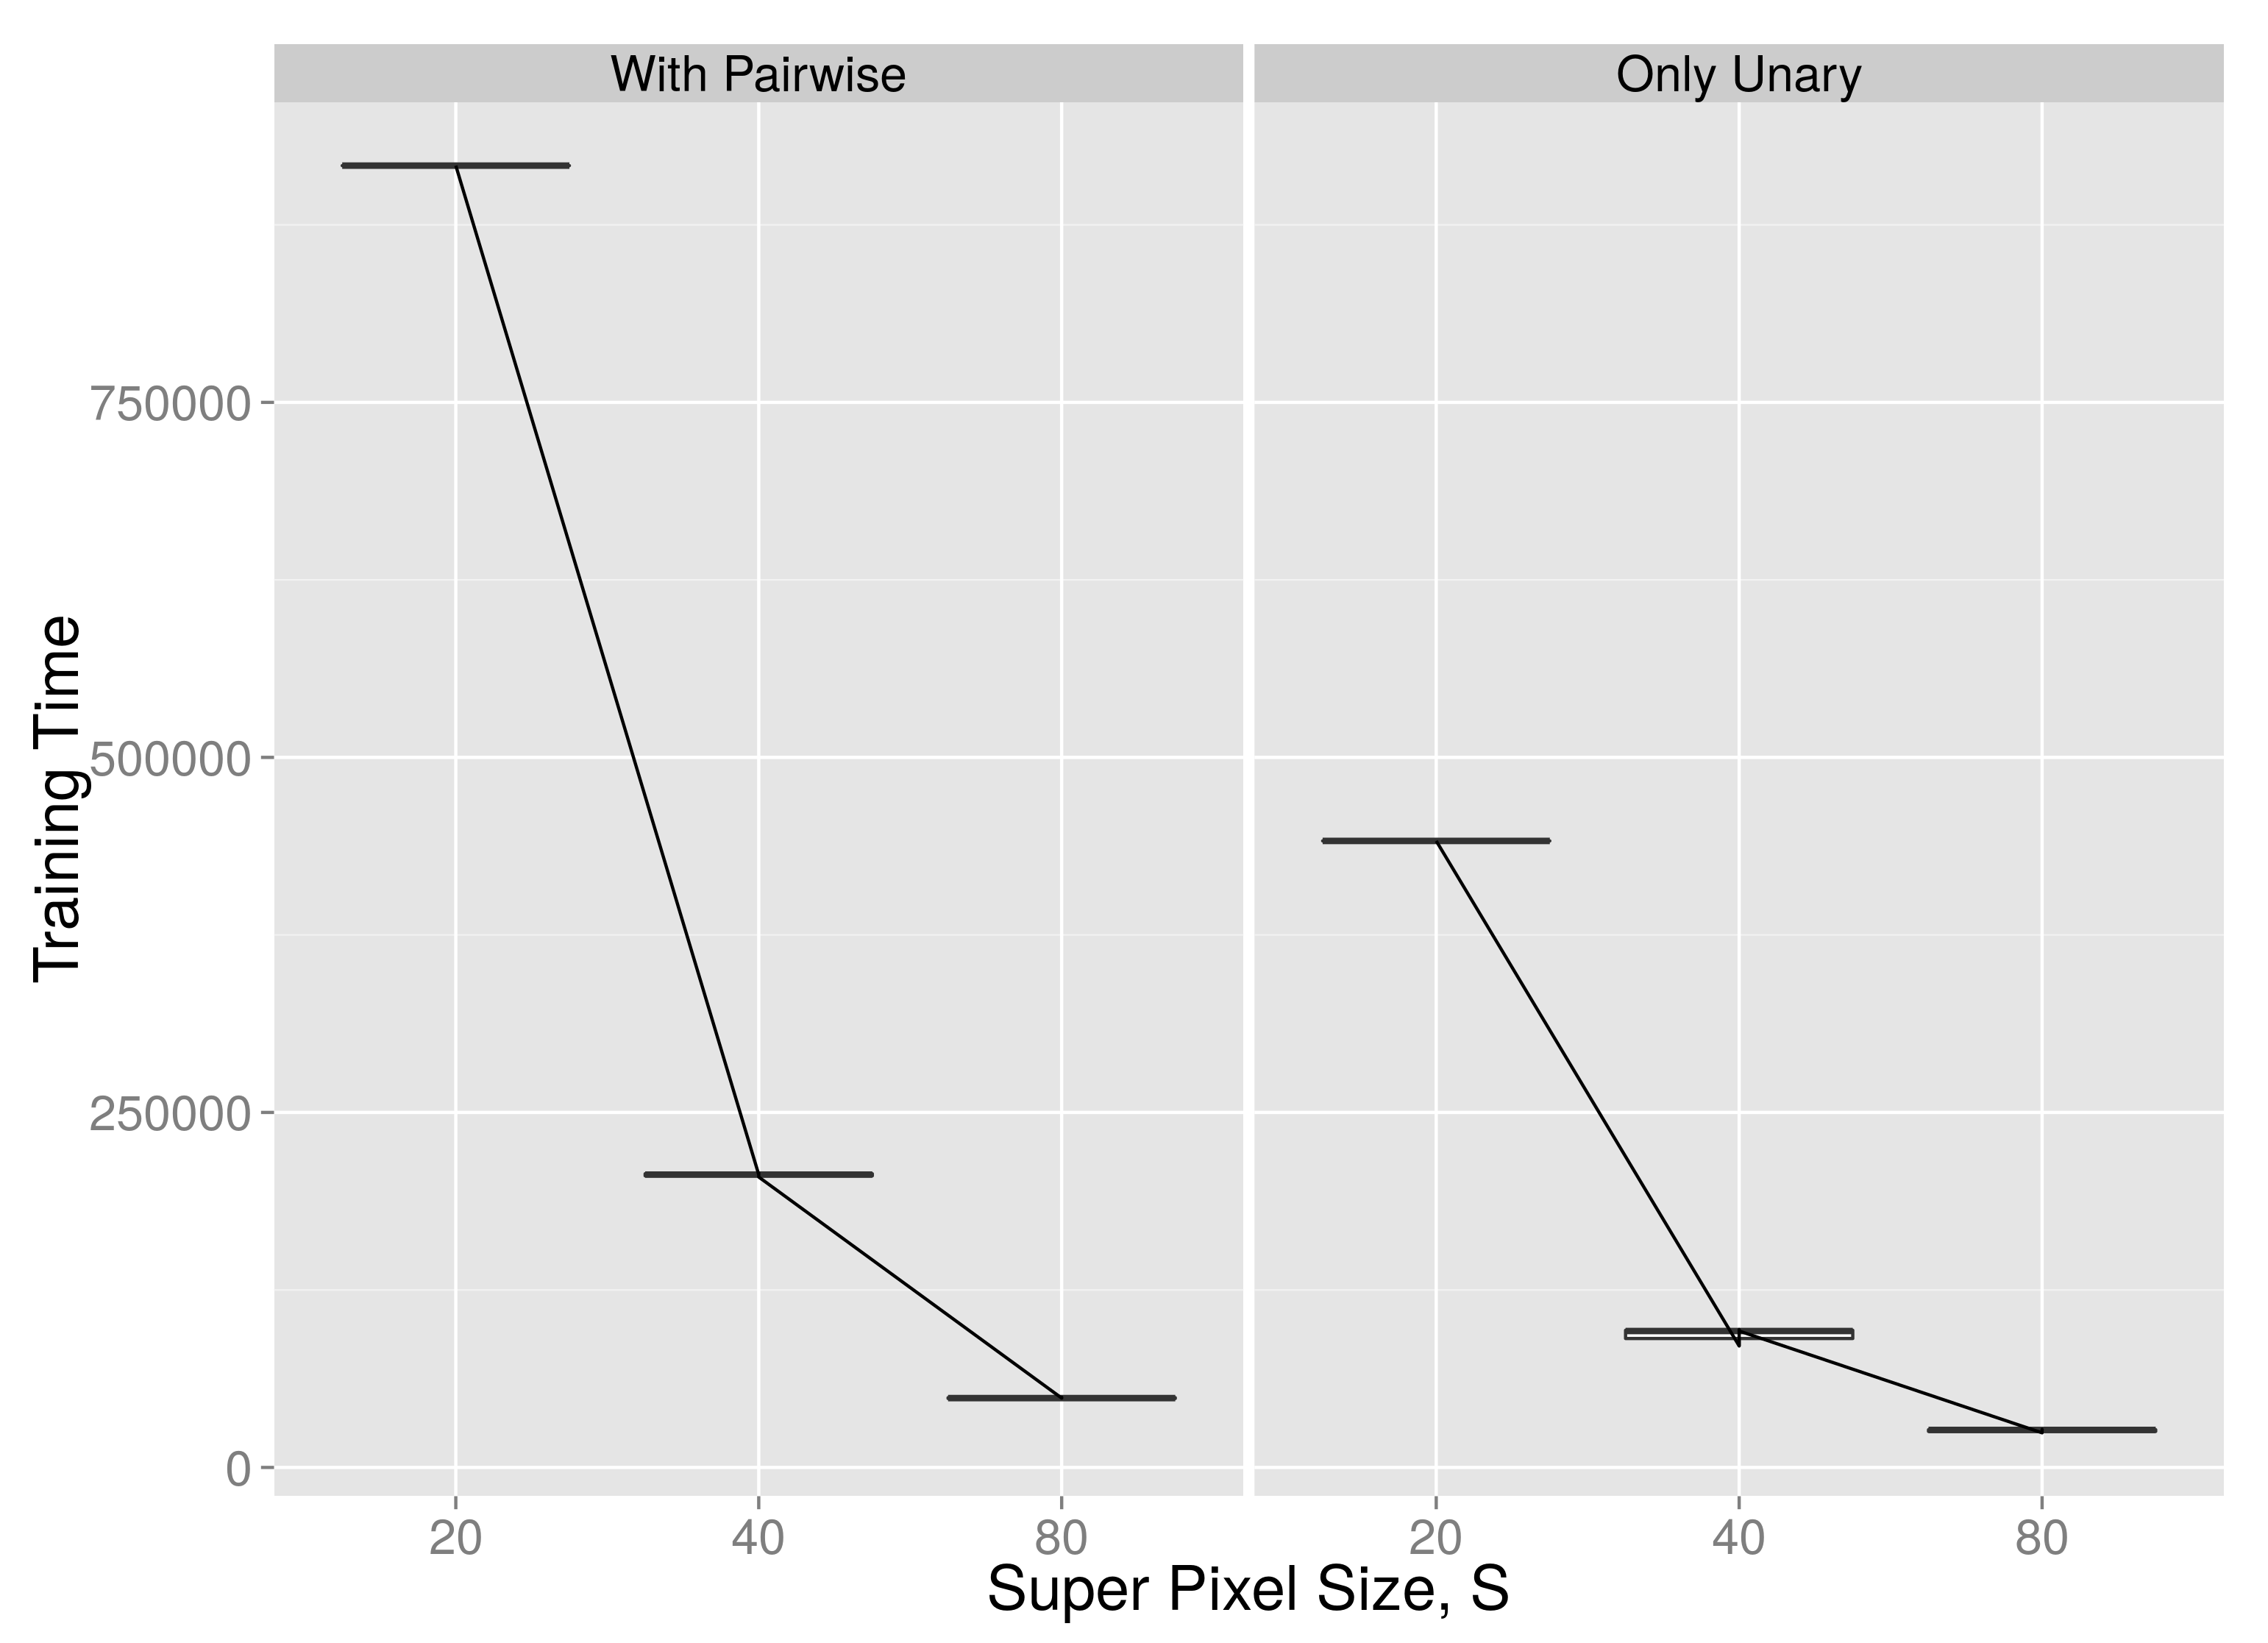
\includegraphics[width=0.8\textwidth]{images/SuperPixel_Speed_up.png}
  \caption{ Here we plot the total training time varying the size of super-pixels (and there fore the number of nodes in the graph). Larger graphs result in larger data volumes moving across the network but the primary time consuming function in our BCFW is the max-oracle. We repeat the same super-pixel resizing experiment with LoopyBP max-oracle and the Naive max for a unary model.} 
  \label{fig:superPixelSpeedup}
\end{figure} 
%



\section{SLIC vs Naive Squares}
When directly comparing the test scores of an SSVM trained on SLIC versus Square super-pixels we found that SLIC does in fact increase performance in both Unary and Pairwise models. 
In contrast to most figures here we are looking at the per pixel loss(see Figure \ref{fig:slicvssquarePix}. The UCSB Nuclei data set is largely skewed towards one class and hence we train on a loss that is weighted by the inverse class frequency. With loss weighting we also find a significant improvement in test loss on this Nuclei dataset, see Figure \ref{fig:slicvssquareNucli}.  


%
\begin{figure}
  \centering
  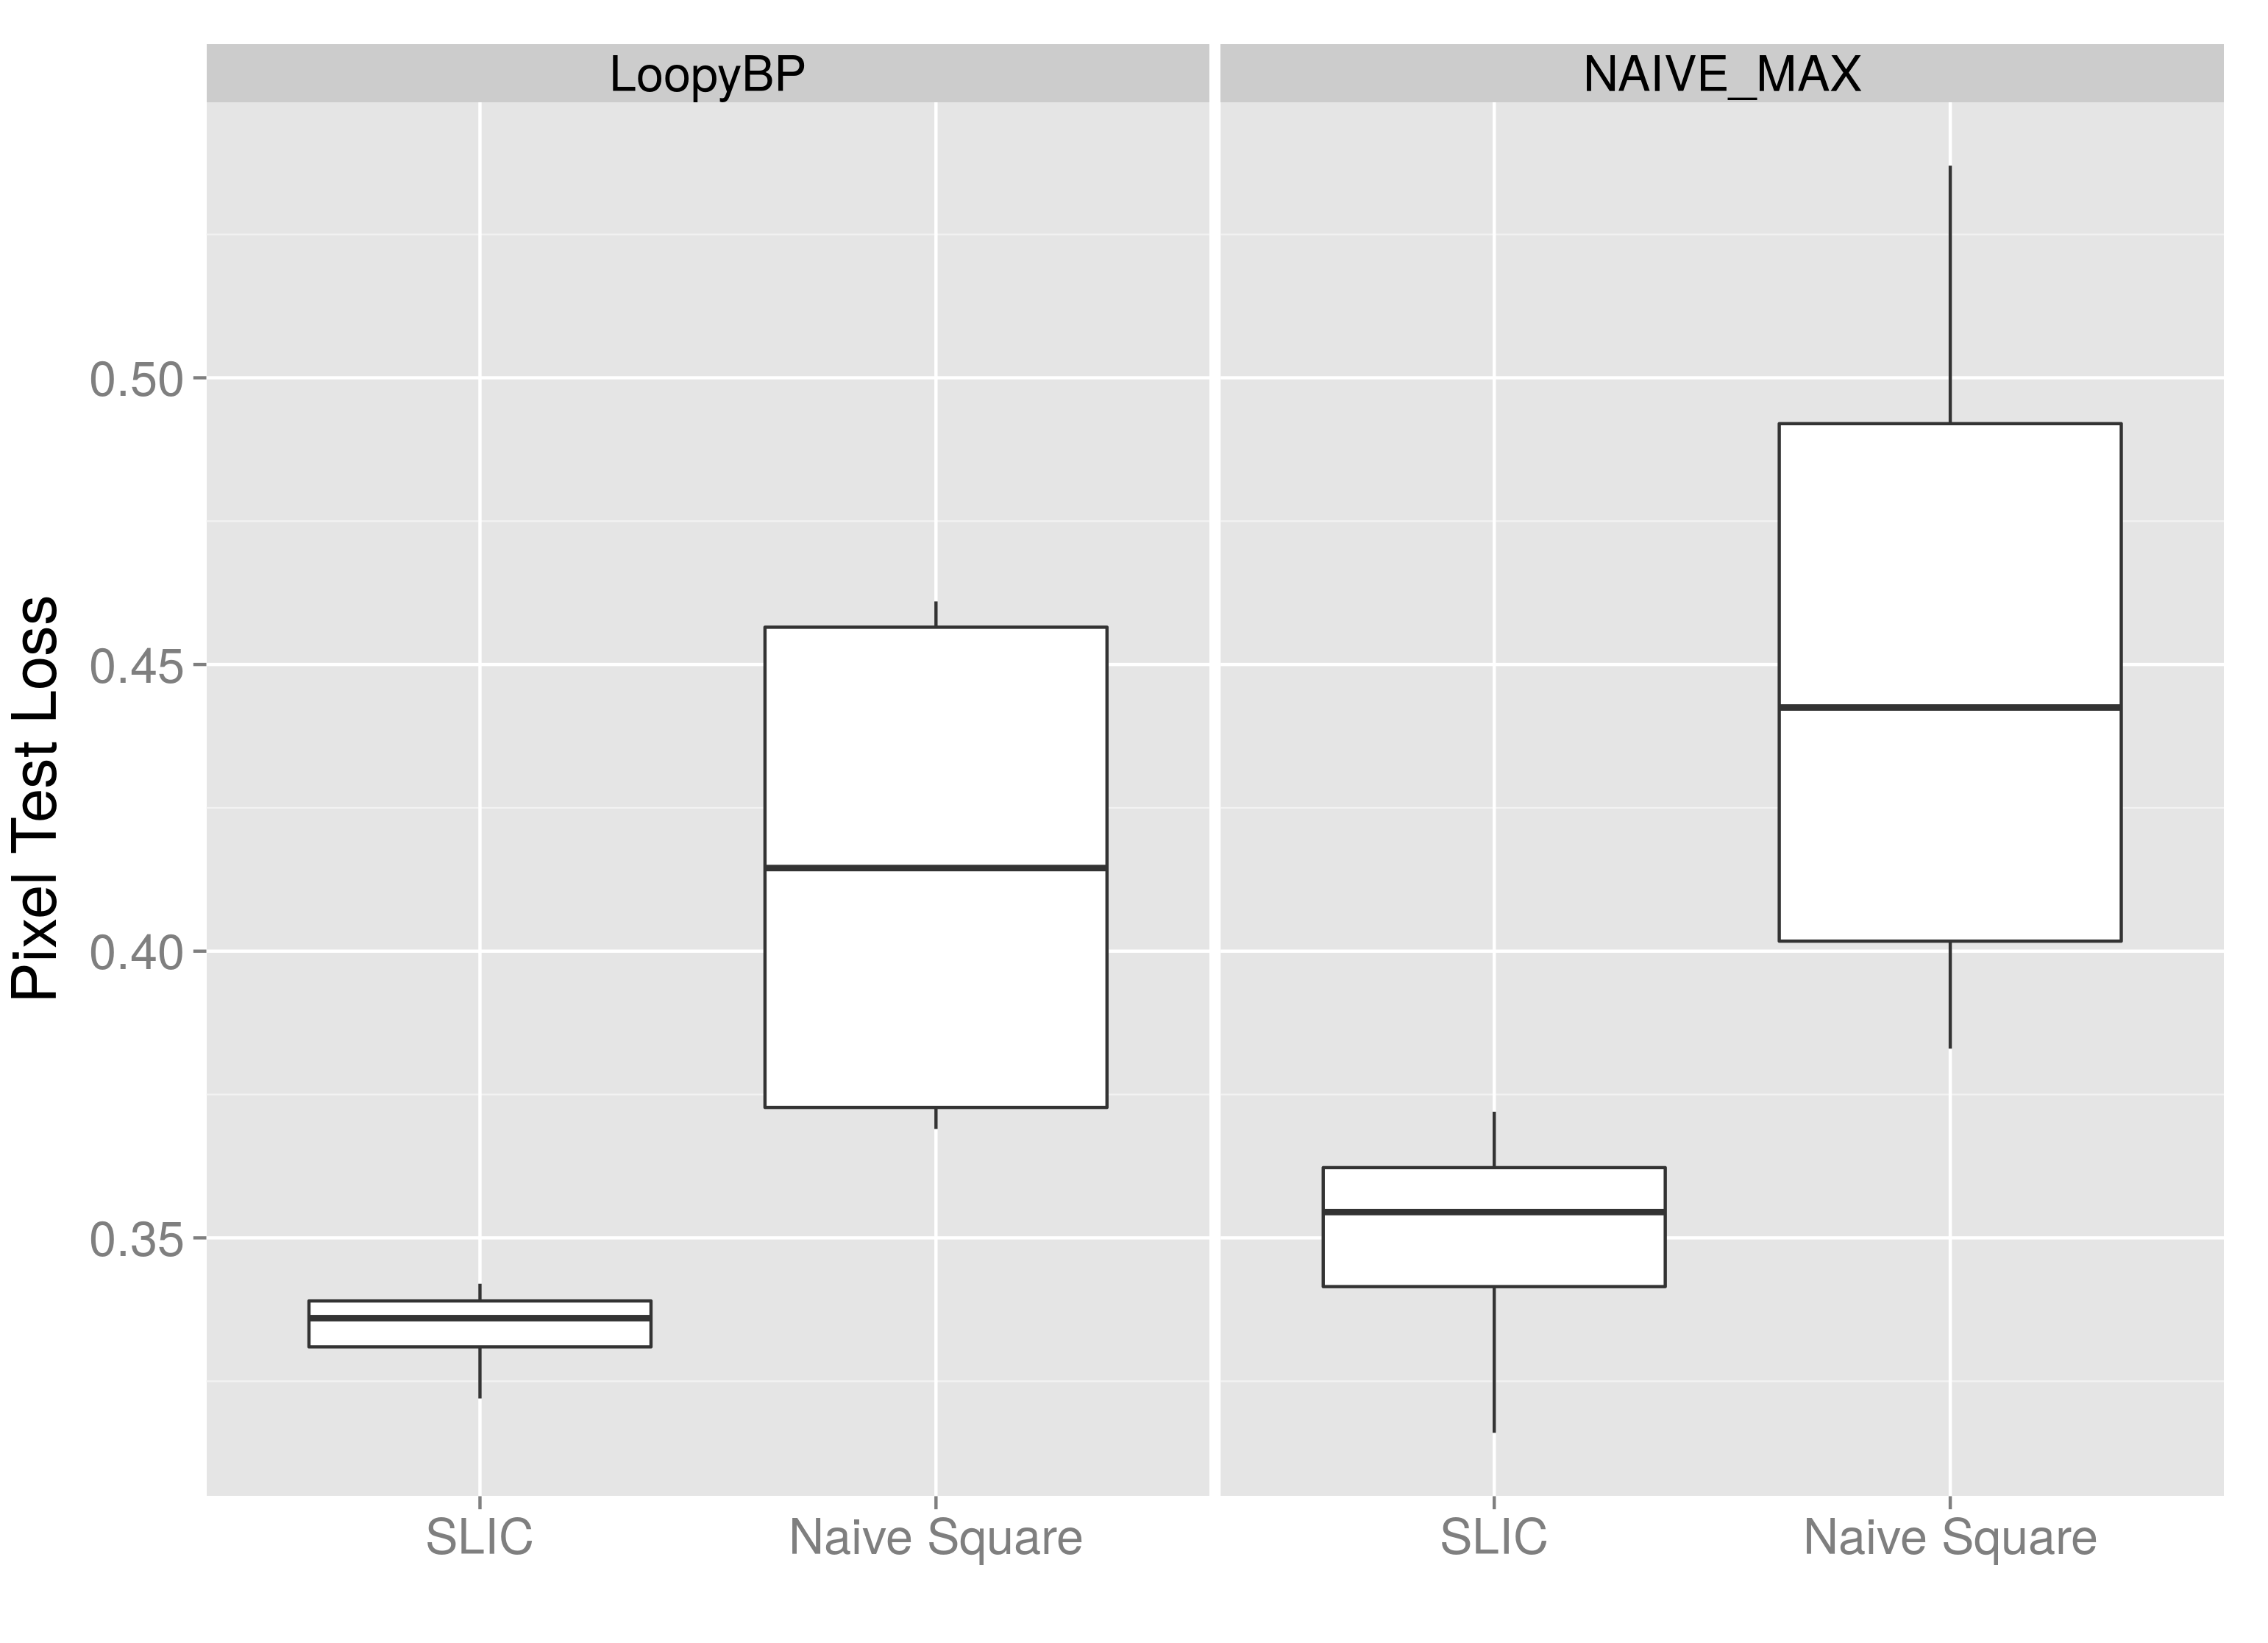
\includegraphics[width=0.8\textwidth]{images/slicVsNaiveSquare_pix_synGen.png}
  \caption{ Comparing the per pixel test loss using either SLIC or Square super-pixels. The experiment was repeated for Unary model and a Pairwise model solved with Loopy Belief Propagation.  Data ( SynthData see \ref{sec:synthDataGen}, WhiteNoise:0.40 SquarImgSize:30 OsilNoise:0.40 SupSqrColorShift:0.0 SuperPix, S:30, M:30, Max Decoding:LoopyBP/NiveMax )  } 
  \label{fig:slicvssquarePix}
\end{figure} 
%


%
\begin{figure}
  \centering
  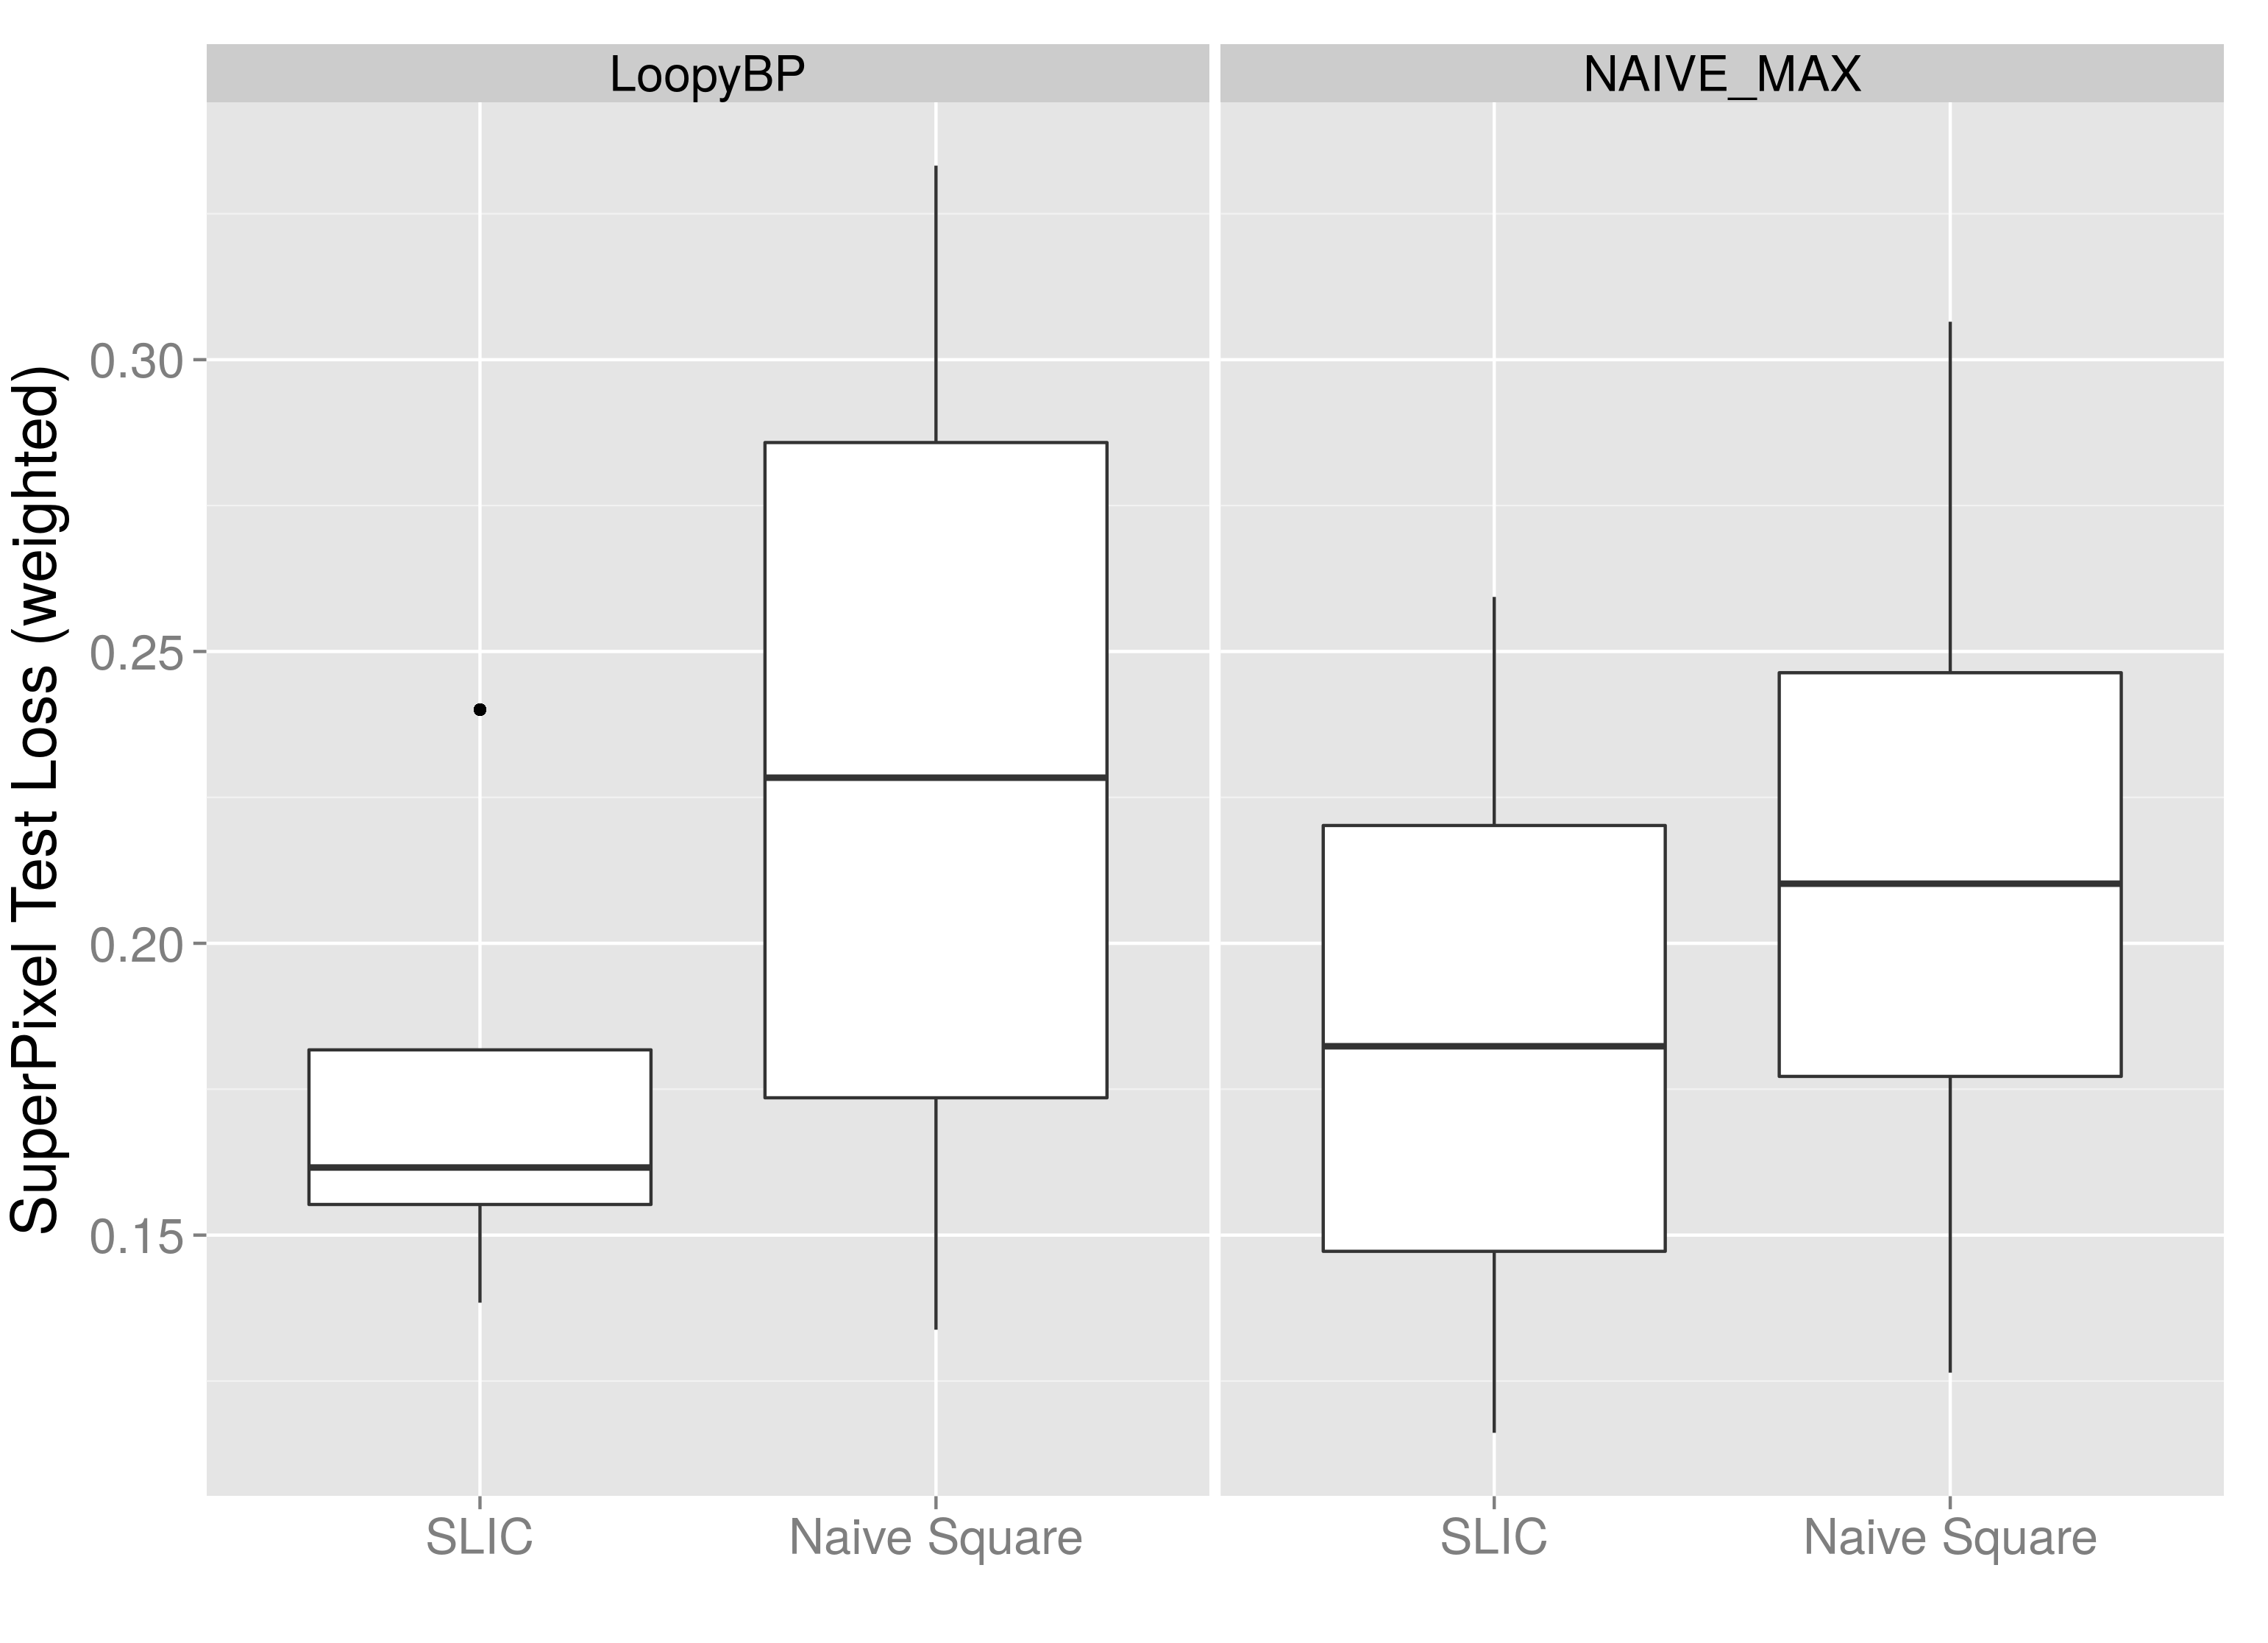
\includegraphics[width=0.8\textwidth]{images/slicVsNaiveSquare_Supx_Nuclei.png}
  \caption{ Comparing the per class frequency per super-pixel test loss using either SLIC or Square super-pixels. The experiment was repeated for Unary model and a Pairwise model solved with Loopy Belief Propagation. Data( Single Channel 3D Nuclei Images \cite{ucsbData}) } 
  \label{fig:slicvssquareNucli}
\end{figure} 
%

\section{Running ScalaSLIC}
ScalaSlic can be used as a standalone package on any kind of data which is saved on spatially located on a uniform grid like color voxels. When constructing a new SLIC() object one needs to input the data in a "Array[Array[Array[DataType]]]" format, where datatype can be an RGB triple, a single grayscale byte but it could also be for example a series of RGB values from a video sequence. While the dataType is technically free from the scala compilers perspective, practically one must be able to define the following functions:  \codeInLine{ distFn:(DataType, DataType) => Double }, which simply measure the distance between two pixels. The functions \codeInLine{rollingAvgFn: ((DataType, DataType, Int) => DataType)} and \codeInLine{normFn: ((DataType, Int) => DataType)} are used for the cluster update step to get an average point in this "DataType" space. For here are the functions we use for RGB  \codeInLine{(a: (Int, Int, Int), b: (Int, Int, Int)) =>  sqrt(Math.pow(a._1 - b._1, 2) + Math.pow(a._2 - b._2, 2) + Math.pow(a._3 - b._3, 2))}, \codeInLine{distFnCol = (a: (Int, Int, Int), b: (Int, Int, Int)) => sqrt(Math.pow(a._1 - b._1, 2) + Math.pow(a._2 - b._2, 2) + Math.pow(a._3 - b._3, 2)) }, \codeInLine{sumFnCol =  (a: (Int, Int, Int), b: (Int, Int, Int)) => ((a._1 + b._1, a._2 + b._2, a._3 + a._3)) } and \codeInLine{normFnCol = (a: (Int, Int, Int), n: Int) => { ((a._1 / n, a._2 / n, a._3 / n))}}. The final mandatory input for ScalaSLIC is \inputArgs{S} which determines the initial grid spacing of the super-pixels and thereby also setting the initial number of cluster centers and partially how large the super-pixels will be. How large the super pixels will be is also modulated by the parameter \inputArgs{M} which specifies the compactness of the super-pixels. If M is not specified we go for the alternative approach of normalizing distances by the max distance in the each super-pixel set. 
\subsection{Visualization SLIC compactness parameters}\label{sec:slicParams}
In our implementation we slightly alter the use of $M$ in contrast to the above distance function. Let $x$,$y$ \& $z$ be vectors containing both pixel coordinates and the spacial centres of the super-pixel clusters index by their subscript. And let $r$, $g$, $b$ be the vectors containing the RGB color information for pixels and super-pixel centres. Here we use subscript $_k$ for some cluster center and subscript $_i$ for some pixel id:   	 $Distance(P,C) = \frac{M^2}{S^2}\sqrt[2]{(x_k -x_i)^2 + (y_k - y_i)^2 + (z_k - z_i)^2} + \sqrt{(r_k - r_i)^2+(g_k - g_i)^2+(b_k - b_i)^2} $. LABColor-space can be used optionally instead of RGB. For an illustration of the effect of parameter $M$ on the segmentation see Figures \ref{fig:showingMonMSRC1}, \ref{fig:showingMonMSRC2} and \ref{fig:showingMonMSRC3}

\begin{figure}[H]
  \centering
  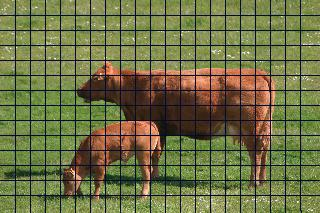
\includegraphics[width=0.7\textwidth,natwidth=610,natheight=642]{images/_supPix_2_15_M0_01_seg.jpg}
  \caption{ SLIC example segmentation on a single 2D MSRC image. With parameters:  S=15, M=1000 } 
  \label{fig:showingMonMSRC1}
\end{figure} 
\begin{figure}[H]
  \centering
  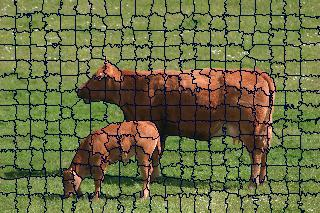
\includegraphics[width=0.7\textwidth,natwidth=610,natheight=642]{images/_supPix_2_15_M5_0_seg.jpg}
  \caption{  SLIC example segmentation on a single 2D MSRC image. With parameters:  S=15, M=45 } 
  \label{fig:showingMonMSRC2}
\end{figure} 
\begin{figure}[H]
  \centering
  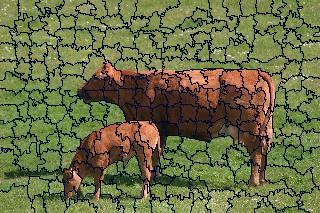
\includegraphics[width=0.7\textwidth,natwidth=610,natheight=642]{images/_supPix_2_15_M10_0_seg.jpg}
  \caption{  SLIC example segmentation on a single 2D MSRC image. With parameters:  S=15, M=14 } 
  \label{fig:showingMonMSRC3}
\end{figure} 

Do to the inherent difficulty of seeing through a block of solid tissue we will visualize the effect of parameter $M$ by only drawing the voxels labelled as foreground, this 3D dataset is a binary classification problem and hence can be displayed like this. 

\begin{figure}[H]
  \centering
  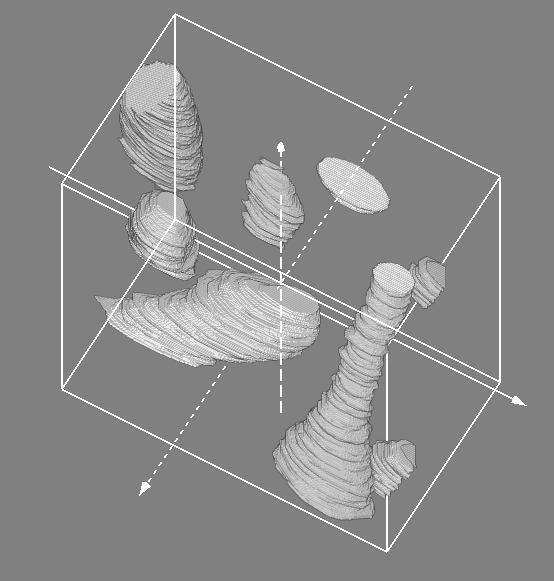
\includegraphics[width=0.7\textwidth]{images/mitochon_groundTruth.png}
  \caption{ The original per pixel ground truth labelling with background transparent and foreground textured to have a surface. Data used in this image is a subset of the EM Mitochondria dataset \cite{mitochondriaData}} 
  \label{fig:showingMmitochonGT}
\end{figure} 
\begin{figure}[H]
  \centering
  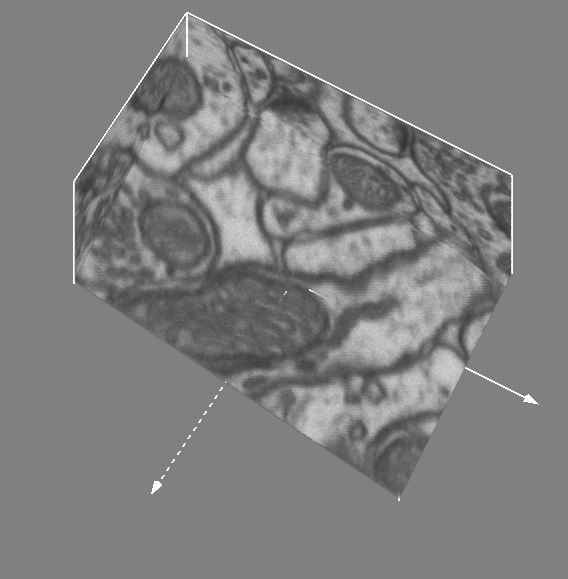
\includegraphics[width=0.7\textwidth]{images/mitochon_original_features.png}
  \caption{ The figure shows a cross sectional cut of the raw data used to construct super-pixels in Figure \ref{fig:showingMmitochonM50} and \ref{fig:showingMmitochonM9}. Data used in this image is a subset of the EM Mitochondria dataset \cite{mitochondriaData}} 
  \label{fig:showingMmitochonRaw}
\end{figure} 

\begin{figure}[H]
  \centering
  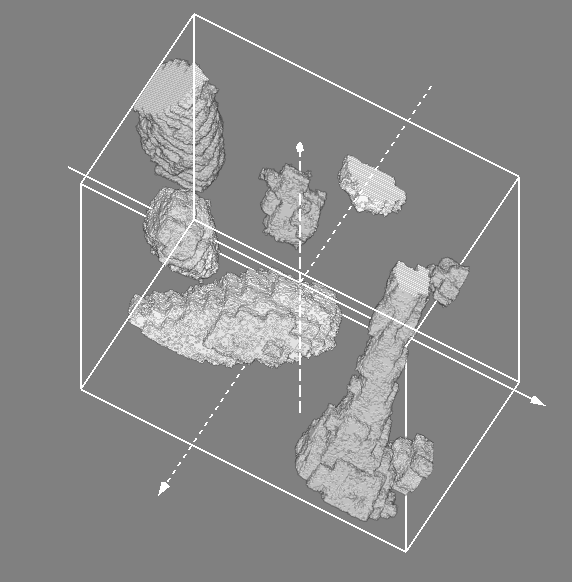
\includegraphics[width=0.7\textwidth]{images/mitochon_s10_m50.png}
  \caption{ The figure shows the textured boundaries of the volume encompassed by the super-pixels which where labelled as being mitochondrial foreground in their graph representation. This image varies from Figure \ref{fig:showingMmitochonM9} in that it used a higher $M=50$The original per pixel ground truth labelling with background transparent and foreground textured to have a surface and hence results in more compact super-pixels. Data used in this image is a subset of the EM Mitochondria dataset \cite{mitochondriaData}} 
  \label{fig:showingMmitochonM50}
\end{figure} 

\begin{figure}[H]
  \centering
  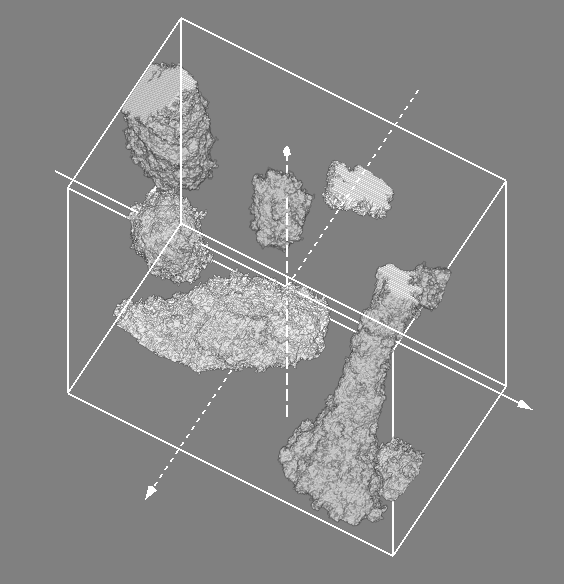
\includegraphics[width=0.7\textwidth]{images/mitochon_s10_m9.png}
  \caption{ The figure shows the textured boundaries of the volume encompassed by the super-pixels which where labelled as being mitochondrial foreground in their graph representation. This image varies from Figure \ref{fig:showingMmitochonM9} in that it used a lower $M=9$ and hence results in less uniformly shaped super-pixels. Data used in this image is a subset of the EM Mitochondria dataset \cite{mitochondriaData}} 
  \label{fig:showingMmitochonM9}
\end{figure} 
